\documentclass{beamer}

% set font
\usepackage{fontspec}
\setmainfont{Noto Serif CJK SC}
\setsansfont{Noto Sans CJK SC}
\setmonofont{Noto Sans Mono CJK SC}

\usepackage{minted}

\usepackage{ctex, hyperref}
\usepackage[T1]{fontenc}

% other packages
\usepackage{latexsym,amsmath,xcolor,multicol,booktabs,calligra}
\usepackage{graphicx,pstricks,listings,stackengine}

\title{操作系统支持矩阵国际化与自动翻译应用}
\subtitle{基于 GPT 模型的自动国际化生成}
\institute{测试小队}
\date{2024 年 7 月 3 日}
\usepackage{Beamer}

% defs
\def\cmd#1{\texttt{\color{red}\footnotesize $\backslash$#1}}
\def\env#1{\texttt{\color{blue}\footnotesize #1}}
\definecolor{deepblue}{rgb}{0,0,0.5}
\definecolor{deepred}{rgb}{0.6,0,0}
\definecolor{deepgreen}{rgb}{0,0.5,0}
\definecolor{halfgray}{gray}{0.55}

\lstset{
    basicstyle=\ttfamily\small,
    keywordstyle=\bfseries\color{deepblue},
    emphstyle=\ttfamily\color{deepred},    % Custom highlighting style
    stringstyle=\color{deepgreen},
    numbers=left,
    numberstyle=\small\color{halfgray},
    rulesepcolor=\color{red!20!green!20!blue!20},
    frame=shadowbox,
}


\begin{document}

\kaishu
\begin{frame}
    \titlepage
\end{frame}

\begin{frame}
    \tableofcontents[sectionstyle=show,subsectionstyle=show/shaded/hide,subsubsectionstyle=show/shaded/hide]
\end{frame}

\section{About}

\begin{frame}{About}
    \begin{itemize}
        \item Github: \href[\@ wychlw]{github.com/wychlw}
        \newline
    \end{itemize}
\end{frame}

\section{Support Matrix}

\begin{frame}{Support Matrix}
    \begin{itemize}
        \item Mainstream operating systems $\times$ Mainstream RISC-V development boards
        \item Installation guide with test results for each combination
        \item \url{ruyisdk.org/supported}
    \end{itemize}
    \begin{figure}
        \centering
            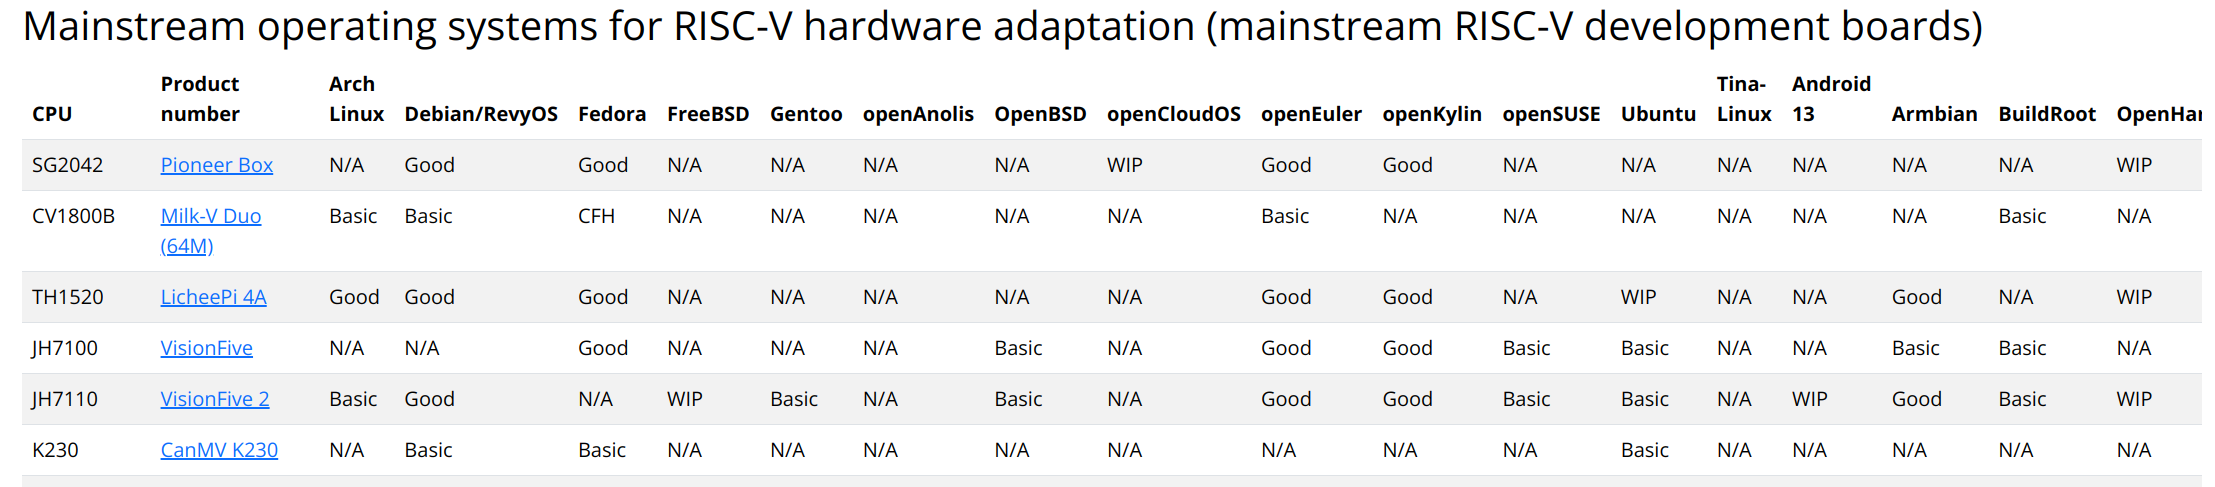
\includegraphics[width=\textwidth]{pic/matrix.png}
    \end{figure}
\end{frame}

\begin{frame}{Support Matrix}
    \begin{itemize}
        \item Check compatibility
        \item All guides in one place
        \item Provide files and scripts
    \end{itemize}
    \begin{figure}
        \centering
            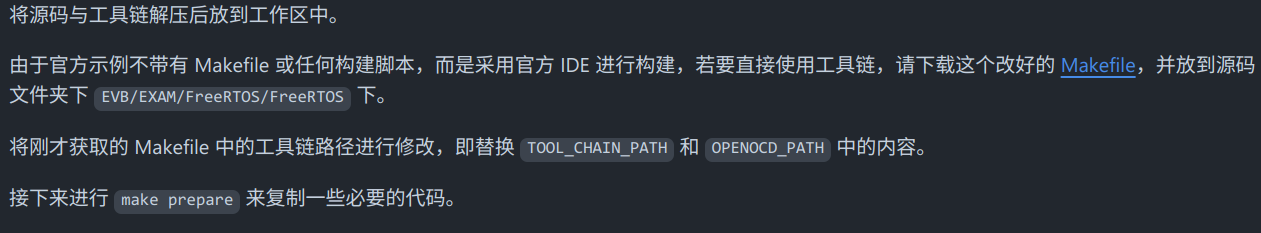
\includegraphics[width=\textwidth]{pic/make_doc.png}
    \end{figure}
\end{frame}

\begin{frame}{Support Matrix}
    \begin{itemize}
        \item Report and fix error
    \end{itemize}
    \begin{figure}
        \centering
            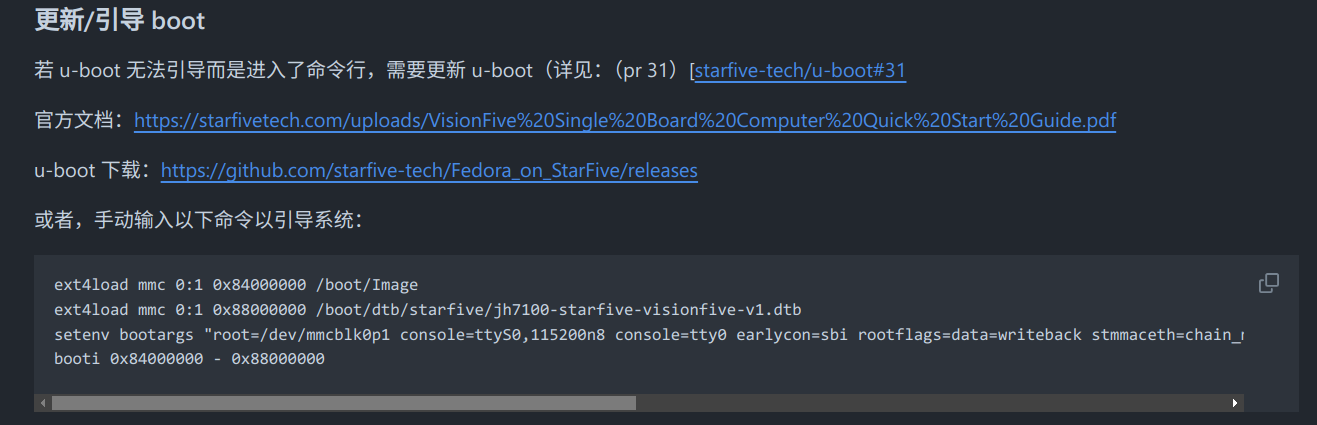
\includegraphics[width=\textwidth]{pic/prob.png}
    \end{figure}
\end{frame}

\begin{frame}{Internationalization And Problems}
    \begin{itemize}
        \item 50 development boards now with approximately 3-4 operating system each \newline
        actually: 219 reports in total
        \item Huge amount of file to be translated: adding a new language is a huge workload without considering the human mistakes
        \item Have some kind of similarity between the reports, but also lots of variations
        \item With technical terms and context
    \end{itemize}
\end{frame}

\section{report-i18n}

\begin{frame}{Ideas of Using LLMs}
    \begin{itemize}
        \item Good quality <-> Traditional doc translation service
        \item Fast and cheap <-> Professional translator
    \end{itemize}
    \bigskip
    \bigskip
    \bigskip
    \bigskip
    \bigskip
\end{frame}

\begin{frame}{Limitation}
    \begin{itemize}
        \item Good quality <-> Traditional doc translation service
        \item Fast and cheap <-> Professional translator
    \end{itemize}
    \bigskip
    But need to pay attention\dots
    \begin{itemize}
        \item Hallucinations
        \item Secretly change minor details
        \item Manual review is still needed
    \end{itemize}
\end{frame}

\begin{frame}{Auto Translation With OpenAI GPT}
    \begin{itemize}
        \item Proj: \url{github.com/wychlw/report-i18n}
        \item Support 3.5 and 4o ( Balance between quality and price )
        \item -- Specialized for test report translation, may need to be adjusted for other purposes
    \end{itemize}
\end{frame}

\begin{frame}{Report i18n}
    \begin{itemize}
        \item Automaticlly translate docs into all target languages
        \item \mintinline{text}|\%s/README.md/README_(lang).md/| , with link changed inside
        \item Will extract everyting in codeblock and not translate them
        \item Will not translate (mostly) URLs
    \end{itemize}
\end{frame}

\begin{frame}{Usage}
    \begin{itemize}
        \item Tweaked model parameters included
        \item Config:
        \begin{itemize}
            \item env.py : API\_KEY and API\_URL 
            \newline OpenAI official and FREE API provided by GPT\_API\_free
            \item conf.py : Config lang and (part of) promote
        \end{itemize}
    \end{itemize}
\end{frame}

\begin{frame}{Usage: conf.py}
    \begin{itemize}
        \item max\_length : Max length for each iteration, generally token size if logogram else $\{3, 4\} * token size$
        \item target\_lang/tips\_translated\_by\_chatgpt : Language to translate to and the tips
        \item model: 4o if logogram to ideogram (or vise versa), else 3.5
        \item template: !important
        \newline eg: 测试成功 -> Test Passed | Test Successful | Test Succeed | Successful Test...
        \newline To regulate general structure of the translation.
    \end{itemize}
\end{frame}

\begin{frame}{Usage: Marker and CI}
    Marker is used to change default behavior (will be removed automatically):
    \begin{itemize}
        \item \mintinline{python3}|r"\[translate\]"| : Force re-translate
        \item \mintinline{python3}|r"\[update\]"| : Force update translation
        \item \mintinline{python3}|r"\[skip_lang\[(.*?)\]\]"| : Skip translate language
        \item Any other good ideas?
    \end{itemize}
    A template for CI, automatically translate and push the repo. (Notice the potential API leak)
\end{frame}

\section{Demo}

\begin{frame}{Demo: report-i18n}
    Let's now try translating a report to French? \\
    (Hopefully the network is good enough)
\end{frame}

\begin{frame}
    \begin{center}
        {\Huge Thanks for your listening!}
    \end{center}
\end{frame}

\end{document}